\section{Minimização de $||\VECTOR{f}(\VECTOR{x})-\VECTOR{b}||_{\MATRIX{C}}^2+\alpha||\VECTOR{x}-\VECTOR{q}||_{\MATRIX{D}}^2$}


\index{Minimização, métodos!Regularização de Tikhonov}
%\index{Problema inverso!Não linear}
\index{Minimização do erro quadrático!Não linear}%!Função $||\VECTOR{f}(\VECTOR{x})-\VECTOR{b}||_{\MATRIX{C}}^2+\alpha||\VECTOR{x}-\VECTOR{q}||_{\MATRIX{D}}^2$}

\begin{theorem}[Solução iterativa]\label{theo:minfxbCfxbaxqaxq}
Dados,
os vetores coluna $\VECTOR{x}\in \mathbb{R}^N$, $\VECTOR{b}\in \mathbb{R}^M$ e $\VECTOR{q}\in \mathbb{R}^N$,  
uma função $\VECTOR{f}:\mathbb{R}^{N} \rightarrow \mathbb{R}^{M}$, 
as matrizes diagonais $\MATRIX{C} \in \mathbb{R}^{M\times M}$ e $\MATRIX{D} \in \mathbb{R}^{N\times N}$, e 
definida a Eq. (\ref{eq:minfxbCfxbaxqaxq1}),
\begin{align}\label{eq:minfxbCfxbaxqaxq1}
e(\VECTOR{x}) &=||\VECTOR{f}(\VECTOR{x})-\VECTOR{b}||_{\MATRIX{C}}^2+\alpha||\VECTOR{x}-\VECTOR{q}||_{\MATRIX{D}}^2\\
              & = (\VECTOR{f}(\VECTOR{x})-\VECTOR{b})^{\transpose}\MATRIX{C}(\VECTOR{f}(\VECTOR{x})-\VECTOR{b})+\alpha(\VECTOR{x}-\VECTOR{q})^{\transpose}\MATRIX{D}(\VECTOR{x}-\VECTOR{q}).
\end{align}
Se desejamos ter o ponto $\VECTOR{\hat{x}}$ que minimiza o escalar $e(\VECTOR{\hat{x}})$,
podemos achar este ponto usando iterativamente a Eq. (\ref{eq:minfxbCfxbaxqaxq2}),
onde  $\MATRIX{J}(\VECTOR{x})$ é a \hyperref[def:jacobian]{\textbf{matriz Jacobiana}}  de $\VECTOR{f}(\VECTOR{x})$.
\begin{equation}\label{eq:minfxbCfxbaxqaxq2}
\VECTOR{x}_{k}\leftarrow \VECTOR{x}_{k-1}-
\left[ \MATRIX{J}(\VECTOR{x}_{k-1})^{\transpose}\MATRIX{C} \MATRIX{J}(\VECTOR{x}_{k-1}) +\alpha\MATRIX{D} \right]^{-1}
 \left\{\MATRIX{J}(\VECTOR{x}_{k-1})^{\transpose}\MATRIX{C}\left[\VECTOR{f}(\VECTOR{x}_{k-1})-\VECTOR{b}\right]+\alpha\MATRIX{D}\left[\VECTOR{x}_{k-1}-\VECTOR{q}\right]\right\}
\end{equation}

Assim, $\VECTOR{\hat{x}}$ pode ser achado 
iniciando a Eq. (\ref{eq:minfxbCfxbaxqaxq2}) desde um $\VECTOR{x}_{0}$ qualquer, 
ate que $\VECTOR{x}_{k}$ seja muito próximo a $\VECTOR{x}_{k-1}$,
onde se declara que $\VECTOR{\hat{x}} \approx \VECTOR{x}_{k}$,
que corresponde a um mínimo\footnote{\label{ref:minfxxq}A
demostração pode ser vista na Prova \ref{proof:theo:minfxbCfxbaxqd}.} de $e(\VECTOR{x})$,
sem aclarar se é local ou global.


\textbf{Considerções:}

\begin{itemize}
\item É interessante verificar na Eq. (\ref{eq:minfxbCfxbaxqaxq2}) 
se  $\MATRIX{J}(\VECTOR{x}_{k-1}=\VECTOR{q}) = \MATRIX{0}$,
pois indica que existe\footref{ref:minfxxq} um ponto de inflexão 
(máximo, mínimo ou ponto de sela) em $e(\VECTOR{x}_{k-1}=\VECTOR{q})$;
consequentemente poderíamos ter achado um mínimo\footnote{\label{foot:labq}É 
interessante verificar o ponto $\VECTOR{q}$, uma vez só, 
antes de iniciar a busca iterativa.}.
\item A busca iterativa da Eq. (\ref{eq:minfxbCfxbaxqaxq2}) é considerada falida quando 
$\MATRIX{J}(\VECTOR{x}_{k-1})^{\transpose}\MATRIX{C} \MATRIX{J}(\VECTOR{x}_{k-1}) +\alpha\MATRIX{D}$
não tem inversa.
\end{itemize}

\end{theorem} 

\begin{tcbattention}
\begin{itemize}
\item O Teorema \ref{theo:minfxbCfxbaxqaxq} pode ser usado para achar o vetor $\VECTOR{x}$
que minimize $e(\VECTOR{x})=||\VECTOR{f}(\VECTOR{x})-\VECTOR{b}||_{\MATRIX{C}}^2+\alpha||\VECTOR{x}-\VECTOR{q}||_{\MATRIX{D}}^2$,
quando sabemos que o vetor $\VECTOR{x}$ que minimiza $||\VECTOR{f}(\VECTOR{x})-\VECTOR{b}||_{\MATRIX{C}}^2$ 
esta perto do ponto $\VECTOR{q}$.
\item No Teorema \ref{theo:minfxbCfxbaxqaxq} o vetor $\VECTOR{x}$ que minimiza $e(\VECTOR{x})$, 
não necessariamente minimiza  $||\VECTOR{f}(\VECTOR{x})-\VECTOR{b}||_{\MATRIX{C}}^2$.
\end{itemize}
\end{tcbattention}

%%%%%%%%%%%%%%%%%%%%%%%%%%%%%%%%%%%%%%%%%%%%%%%%%%%%%%%%%%%%%%%%%%%%%%%%%%%%%%%%
\subsection{Exemplos de minimização de 
$||\VECTOR{f}(\VECTOR{x})-\VECTOR{b}||_{\MATRIX{C}}^2+\alpha||\VECTOR{x}-\VECTOR{q}||_{\MATRIX{D}}^2$}


\begin{example}[Quando existem muitos mínimos locais e um
$\VECTOR{\hat{x}}$ que cumpre que $\VECTOR{f}(\VECTOR{\hat{x}}) \approx \VECTOR{b}$:]
\label{ex:minfxbCfxbaxqaxq1}
Conhecida um escalar $\alpha$, uma função $\VECTOR{f}(\VECTOR{x}) : \mathbb{R}^{2} \rightarrow \mathbb{R}^{3}$,
um ponto $\VECTOR{q}$
é outro ponto $\VECTOR{b}$, no domínio e no contradomínio de $\VECTOR{f}(\VECTOR{x})$, respetivamente;
achar o valor $\VECTOR{\hat{x}}$ que minimize 
$||\VECTOR{f}(\VECTOR{x})-\VECTOR{b}||_{\MATRIX{C}}^2+\alpha||\VECTOR{x}-\VECTOR{q}||_{\MATRIX{D}}^2$;
sabendo que:
\begin{equation}
\VECTOR{b}=\begin{bmatrix}
1\\
1\\
2
\end{bmatrix},
\qquad 
\VECTOR{f}(\VECTOR{x})=\begin{bmatrix}
sin(\frac{x_1 5 \pi}{2})\\
sin(\frac{x_2 5 \pi}{2})\\
x_1+x_2
\end{bmatrix},
\qquad
\alpha=0.1,
\qquad
\VECTOR{q}=\begin{bmatrix}
0\\
0\\
0
\end{bmatrix}.
\end{equation}
Com esta informação podemos calcular o jacobiano $\MATRIX{J}(\VECTOR{x})$ de $\VECTOR{f}(\VECTOR{x})$,
 e escolher as matrizes $\MATRIX{C} \in \mathbb{R}^{3}$ e $\MATRIX{D} \in \mathbb{R}^{2}$, 
com elementos iguais à  matriz identidade. 
Assim, usando a Eq. (\ref{eq:minfxbCfxbaxqaxq1}),
obtemos a superfície $e(\VECTOR{x})$ como mostra a Figura \ref{fig:ex:minfxbCfxbaxqaxq3:a}.
Podemos ver as respostas a este exemplo na Solução \ref{ex:minfxbCfxbaxqaxq3:sol1} e \ref{ex:minfxbCfxbaxqaxq3:sol2}.
\end{example}

\begin{SolutionT}[Relativa ao Exemplo \ref{ex:minfxbCfxbaxqaxq1}:]
\label{ex:minfxbCfxbaxqaxq3:sol1}
Se escolhemos o ponto inicial $\VECTOR{x}_0=[2\quad 2]^{\transpose}$,
com pendente\footnote{O cálculo da
pendente de $e(\VECTOR{\hat{x}})$ pode ser visto no Teorema \ref{theo:derfxbCfxb0}.} 
$\frac{\partial e(\VECTOR{x}_0)}{\partial \VECTOR{x} }=[20.108\quad 20.108]^{\transpose}$ e 
usamos iterativamente a Eq. (\ref{eq:minfxbCfxbaxqaxq2}), obtemos os valores 
de $\VECTOR{x}_k$ e $e(\VECTOR{x}_k)$, como mostra a Tabela \ref{table:ex:minfxbCfxbaxqaxq3},
onde se assume o final do processo iterativo quando $\VECTOR{x}_k \approx \VECTOR{x}_{k-1}$.
Assim, a aproximação iterativa conclui na resposta 
$\VECTOR{\hat{x}}\approx \VECTOR{x}_{7} =[1.7013\quad 1.7013]^{\transpose}$
com um erro $e(\VECTOR{\hat{x}})=2.7094$ e uma pendente
$\frac{\partial e(\VECTOR{\hat{x}})}{\partial \VECTOR{x} }=[0.0016997\quad 0.0016997]^{\transpose}$
pequena;
este processo pode ser visto de forma gráfica na Figura \ref{fig:ex:minfxbCfxbaxqaxq3:b}.
\end{SolutionT}

\begin{table}[h!]
\centering
\begin{tabular}{|l|l|l|l|l|l|l|l|l|}
\hline
$k$ & 0 & 1 & 2 & 3 & 4 & 5 & 6 & 7\\ \hline
$\VECTOR{x}_k$ & 2.0000 & 1.8424 & 1.6110 & 1.7021 & 1.7009 & 1.7014 & 1.7012 & 1.7013 \\ 
~              & 2.0000 & 1.8424 & 1.6110 & 1.7021 & 1.7009 & 1.7014 & 1.7012 & 1.7013 \\ \hline
$||\VECTOR{x}_k||$ & 2.8284 & 2.6055 & 2.2782 & 2.4071 & 2.4055 & 2.4061 & 2.4059 & 2.4060 \\ \hline
$e(\VECTOR{x}_k)$ & 6.8000 & 3.5233 & 3.6832 & 2.7095 & 2.7094 & 2.7094 & 2.7094 & 2.7094 \\ \hline
\end{tabular}
\caption{Resposta iterativa do Exemplo \ref{ex:minfxbCfxbaxqaxq1}.}
\label{table:ex:minfxbCfxbaxqaxq3}
\end{table}
\begin{figure}[h!]
     \centering
     \begin{subfigure}[b]{0.49\textwidth}
         \centering
         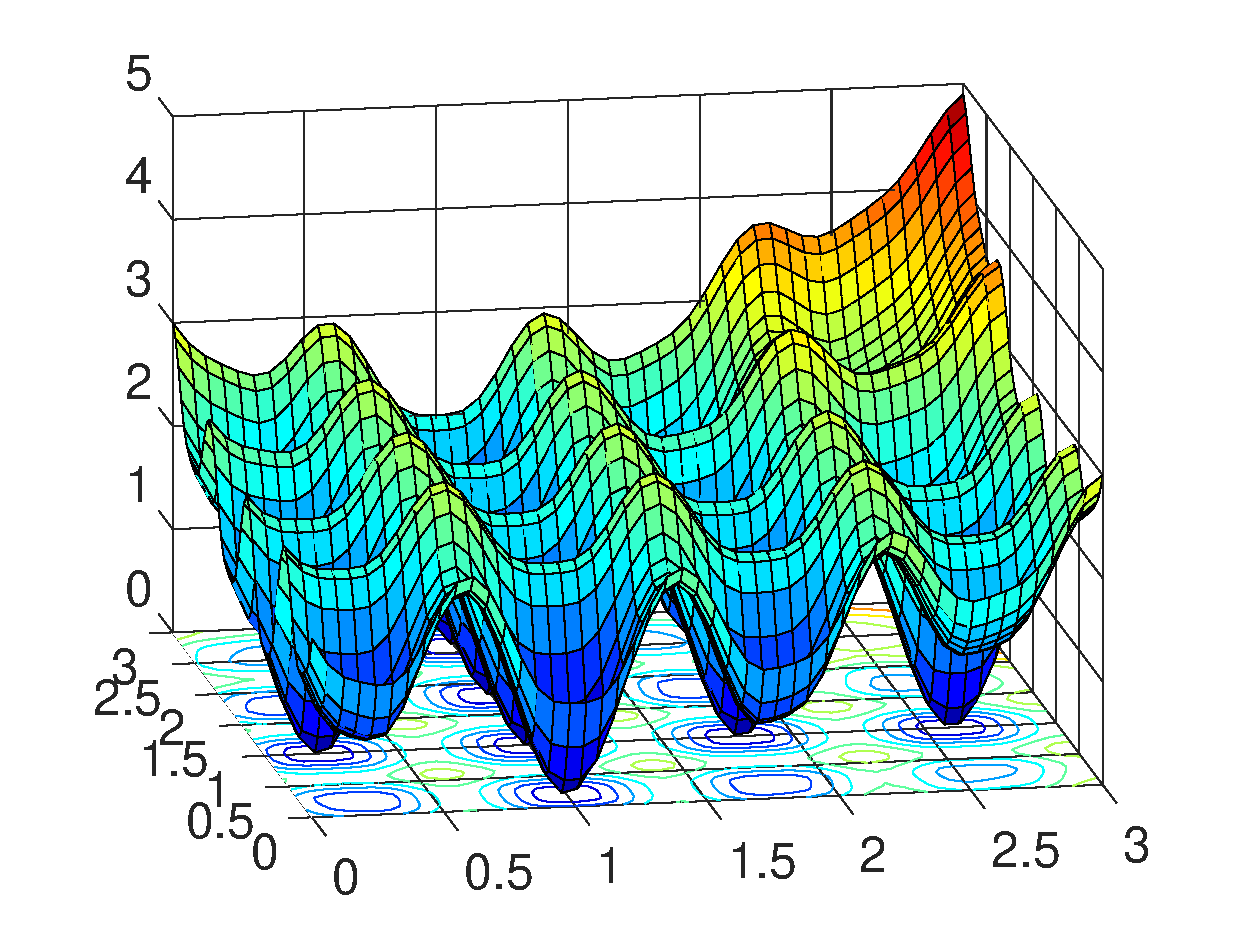
\includegraphics[width=0.98\textwidth]{chapters/minimization-fx/mfiles/fxxq3/surfcfx3.eps}
         \caption{Superficie $e(\VECTOR{x})$. }
         \label{fig:ex:minfxbCfxbaxqaxq3:a}
     \end{subfigure}
     \hfill
     \begin{subfigure}[b]{0.49\textwidth}
         \centering
         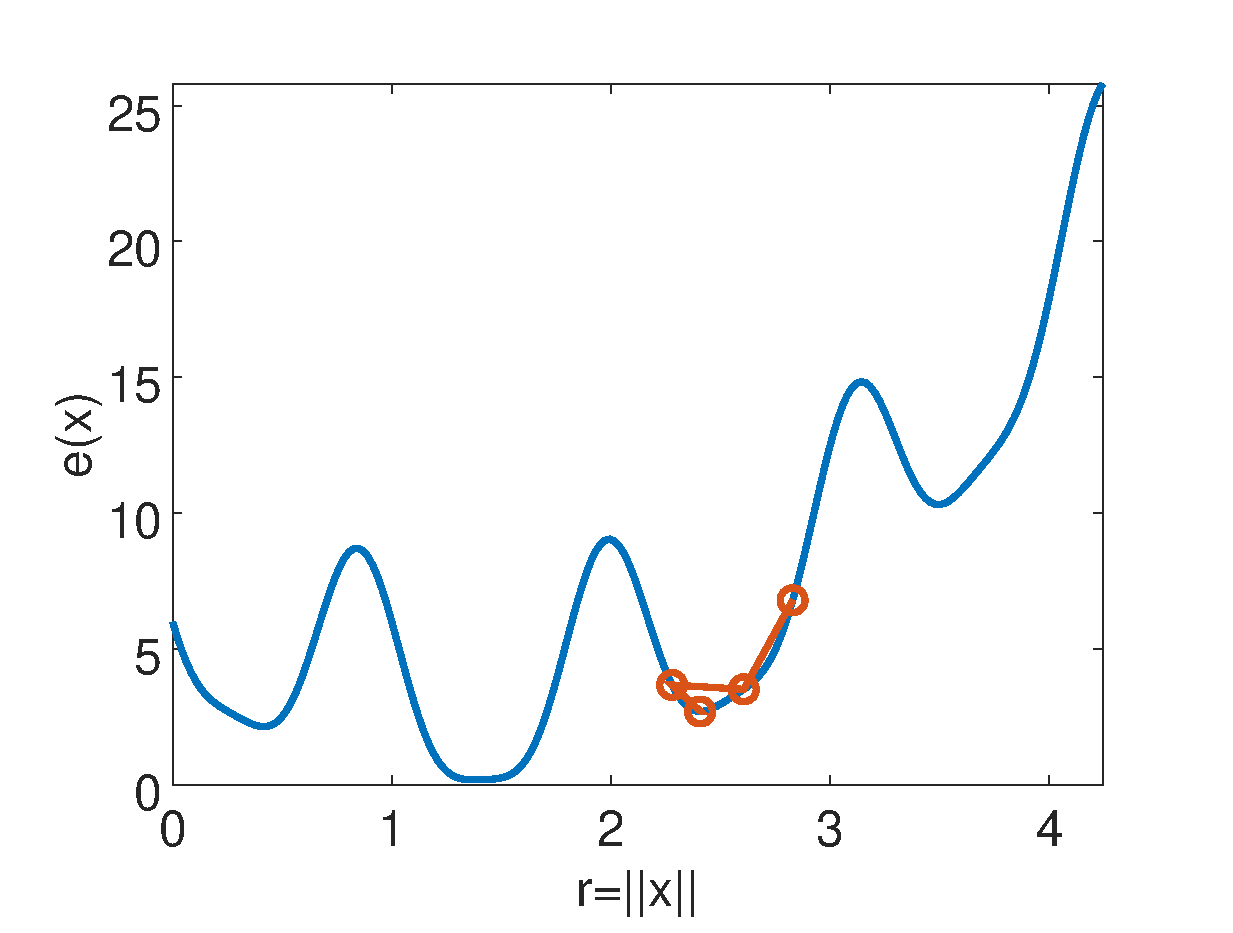
\includegraphics[width=0.98\textwidth]{chapters/minimization-fx/mfiles/fxxq3/plotfx3.eps}
         \caption{Curva $e(\VECTOR{x})$ na direção $(1,1)$.}
         \label{fig:ex:minfxbCfxbaxqaxq3:b}
     \end{subfigure}
        \caption{Resposta gráfica do Exemplo \ref{ex:minfxbCfxbaxqaxq1}. }
        \label{fig:ex:minfxbCfxbaxqaxq3}
\end{figure}

\begin{SolutionT}[Relativa ao Exemplo \ref{ex:minfxbCfxbaxqaxq1}:]
\label{ex:minfxbCfxbaxqaxq3:sol2}
Se escolhemos o ponto inicial $\VECTOR{x}_0=[\frac{11.0999}{5}$ $\frac{11.0999}{5}]^{\transpose}$,
com pendente\footnote{O cálculo da
pendente de $e(\VECTOR{\hat{x}})$ pode ser visto no Teorema \ref{theo:derfxbCfxb0}.} 
$\frac{\partial e(\VECTOR{x}_0)}{\partial \VECTOR{x} }=[0.44442\quad 0.44442]^{\transpose}$ e 
usamos iterativamente a Eq. (\ref{eq:minfxbCfxbaxqaxq2}), obtemos os valores 
de $\VECTOR{x}_k$ e $e(\VECTOR{x}_k)$, como mostra a Tabela \ref{table:ex:minfxbCfxbaxqaxq4},
onde se assume o final do processo iterativo quando $\VECTOR{x}_k \approx \VECTOR{x}_{k-1}$.
Assim, a aproximação iterativa conclui na resposta 
$\VECTOR{\hat{x}}\approx \VECTOR{x}_{7} =[0.97172\quad 0.97172]^{\transpose}$
com um erro $e(\VECTOR{\hat{x}})=0.19325$ e uma pendente
$\frac{\partial e(\VECTOR{\hat{x}})}{\partial \VECTOR{x} }=[-0.0037461\quad -0.0037461]^{\transpose}$
pequena;
este processo pode ser visto de forma gráfica na Figura \ref{fig:ex:minfxbCfxbaxqaxq4:b}.
\end{SolutionT}


\begin{table}[h!]
\centering
\begin{tabular}{|l|l|l|l|l|l|l|l|l|}
\hline
$k$ & 0 & 1 & 2 & 3 & 4 & 5 & 6 & 7\\ \hline
$\VECTOR{x}_k$ & 2.21998 & 2.15837 & 1.27881 & 1.02790 & 0.98814 & 0.96083 & 0.97294 & 0.97172 \\ 
~              & 2.21998 & 2.15837 & 1.27881 & 1.02790 & 0.98814 & 0.96083 & 0.97294 & 0.97172 \\ \hline
$||\VECTOR{x}_k||$ & 3.1395 & 3.0524 & 1.8085 & 1.4537 & 1.3974 & 1.3588 & 1.3759 & 1.3742 \\ \hline
$e(\VECTOR{x}_k)$ & 14.84107 & 13.88071 & 5.63225 & 0.21557 & 0.19588 & 0.19518 & 0.19326 & 0.19325 \\ \hline
\end{tabular}
\caption{Resposta iterativa do Exemplo \ref{ex:minfxbCfxbaxqaxq1}.}
\label{table:ex:minfxbCfxbaxqaxq4}
\end{table}

     \begin{figure}[!h]
         \centering
         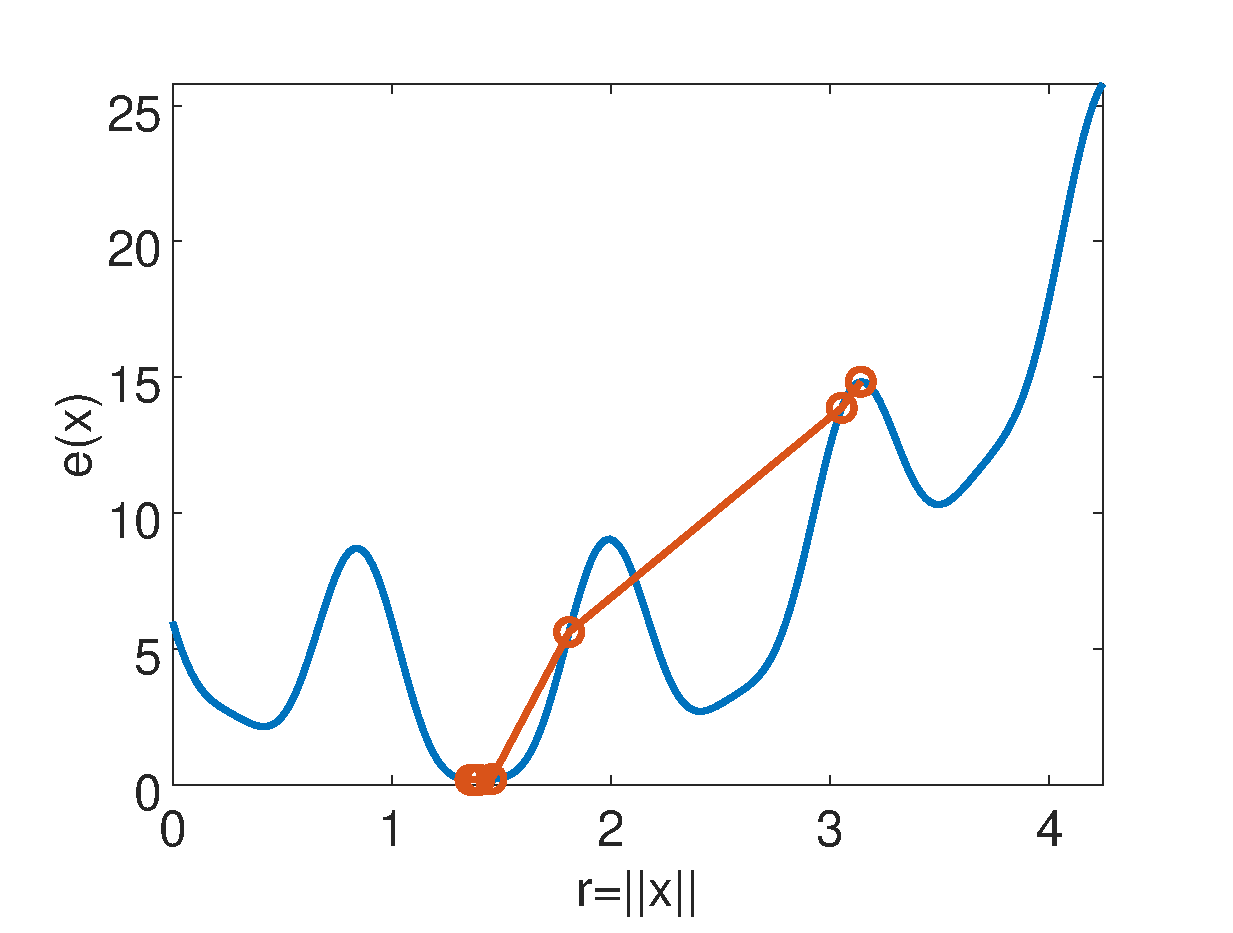
\includegraphics[width=0.5\textwidth]{chapters/minimization-fx/mfiles/fxxq3/plotfx4.eps}
         \caption{Curva $e(\VECTOR{x})$ na direção $(1,1)$.}
         \label{fig:ex:minfxbCfxbaxqaxq4:b}
     \end{figure}


